
\documentclass[11pt]{article}\usepackage[]{graphicx}\usepackage[]{xcolor}
% maxwidth is the original width if it is less than linewidth
% otherwise use linewidth (to make sure the graphics do not exceed the margin)
\makeatletter
\def\maxwidth{ %
  \ifdim\Gin@nat@width>\linewidth
    \linewidth
  \else
    \Gin@nat@width
  \fi
}
\makeatother

\definecolor{fgcolor}{rgb}{0.345, 0.345, 0.345}
\newcommand{\hlnum}[1]{\textcolor[rgb]{0.686,0.059,0.569}{#1}}%
\newcommand{\hlstr}[1]{\textcolor[rgb]{0.192,0.494,0.8}{#1}}%
\newcommand{\hlcom}[1]{\textcolor[rgb]{0.678,0.584,0.686}{\textit{#1}}}%
\newcommand{\hlopt}[1]{\textcolor[rgb]{0,0,0}{#1}}%
\newcommand{\hlstd}[1]{\textcolor[rgb]{0.345,0.345,0.345}{#1}}%
\newcommand{\hlkwa}[1]{\textcolor[rgb]{0.161,0.373,0.58}{\textbf{#1}}}%
\newcommand{\hlkwb}[1]{\textcolor[rgb]{0.69,0.353,0.396}{#1}}%
\newcommand{\hlkwc}[1]{\textcolor[rgb]{0.333,0.667,0.333}{#1}}%
\newcommand{\hlkwd}[1]{\textcolor[rgb]{0.737,0.353,0.396}{\textbf{#1}}}%
\let\hlipl\hlkwb

\usepackage{framed}
\makeatletter
\newenvironment{kframe}{%
 \def\at@end@of@kframe{}%
 \ifinner\ifhmode%
  \def\at@end@of@kframe{\end{minipage}}%
  \begin{minipage}{\columnwidth}%
 \fi\fi%
 \def\FrameCommand##1{\hskip\@totalleftmargin \hskip-\fboxsep
 \colorbox{shadecolor}{##1}\hskip-\fboxsep
     % There is no \\@totalrightmargin, so:
     \hskip-\linewidth \hskip-\@totalleftmargin \hskip\columnwidth}%
 \MakeFramed {\advance\hsize-\width
   \@totalleftmargin\z@ \linewidth\hsize
   \@setminipage}}%
 {\par\unskip\endMakeFramed%
 \at@end@of@kframe}
\makeatother

\definecolor{shadecolor}{rgb}{.97, .97, .97}
\definecolor{messagecolor}{rgb}{0, 0, 0}
\definecolor{warningcolor}{rgb}{1, 0, 1}
\definecolor{errorcolor}{rgb}{1, 0, 0}
\newenvironment{knitrout}{}{} % an empty environment to be redefined in TeX

\usepackage{alltt}

% Packages for graphics & layout
\usepackage{graphicx}
\usepackage{epstopdf}
\usepackage{caption}
\usepackage{subcaption}
\usepackage{booktabs}
\usepackage[a4paper,margin=0.5in]{geometry}
\usepackage{lipsum}
\usepackage{multicol}

\usepackage[utf8]{inputenc}
\usepackage{enumitem}

% Packages for math
\usepackage{amsmath}
\usepackage{amsfonts}
\usepackage{amssymb}

% Package for bibliography
\usepackage{natbib}
\usepackage{hyperref}

% listing setup \usepackage{listings}
\usepackage{color} % For syntax highlighting color
\captionsetup{labelfont=bf}
\setlength{\parskip}{0.5\baselineskip}


\title{\textbf{Data Analysis Practice}}
\author{Michael V Cumbo}
\date{\today}
\IfFileExists{upquote.sty}{\usepackage{upquote}}{}
\begin{document}
\maketitle
\begin{knitrout}
\definecolor{shadecolor}{rgb}{0.969, 0.969, 0.969}\color{fgcolor}\begin{kframe}
\begin{alltt}
\hlkwd{library}\hlstd{(tidyverse)}
\hlkwd{library}\hlstd{(lubridate)}
\hlkwd{library}\hlstd{(RSQLite)}
\hlkwd{library}\hlstd{(DBI)}
\hlkwd{library}\hlstd{(ggplot2)}
\hlkwd{library}\hlstd{(dplyr)}
\hlkwd{library}\hlstd{(forcats)}
\hlkwd{library}\hlstd{(GGally)}
\hlkwd{library}\hlstd{(stringr)}
\hlkwd{library}\hlstd{(magrittr)}

\hlkwd{setwd}\hlstd{(}\hlstr{"~/workbook"}\hlstd{)}
\hlstd{con} \hlkwb{<-} \hlkwd{dbConnect}\hlstd{(RSQLite}\hlopt{::}\hlkwd{SQLite}\hlstd{(),} \hlstr{"Disaster_Data.db"}\hlstd{)}
\hlkwd{dbListTables}\hlstd{(con)}
\end{alltt}
\begin{verbatim}
## [1] "US_Declarations_2023"     "sqlean_define"           
## [3] "us_disaster_declarations"
\end{verbatim}
\begin{alltt}
\hlstd{declarations_2023} \hlkwb{<-} \hlkwd{as_tibble}\hlstd{(}\hlkwd{dbGetQuery}\hlstd{(}
  \hlstd{con,}
  \hlstr{"SELECT
  disasterNumber,
  state,
  declarationType,
  incidentType,
  declarationDate
  FROM US_Declarations_2023
ORDER BY declarationDate;"}
\hlstd{))}
\hlkwd{dbDisconnect}\hlstd{(con)}
\end{alltt}
\end{kframe}
\end{knitrout}

\begin{knitrout}
\definecolor{shadecolor}{rgb}{0.969, 0.969, 0.969}\color{fgcolor}\begin{kframe}
\begin{alltt}
\hlstd{annual_disasters} \hlkwb{<-} \hlstd{declarations_2023} \hlopt
  \hlkwd{filter}\hlstd{(}\hlopt{!}\hlstd{Year} \hlopt \hlkwd{c}\hlstd{(}\hlnum{2020}\hlstd{,} \hlnum{2005}\hlstd{,} \hlnum{2024}\hlstd{),}
         \hlstd{declarations_2023}\hlopt{$}\hlstd{incidentType} \hlopt{!=} \hlstr{"Biological"}\hlstd{)} \hlopt
  \hlkwd{group_by}\hlstd{(Year)} \hlopt
  \hlkwd{summarise}\hlstd{(}\hlkwc{DisasterCount} \hlstd{=} \hlkwd{n}\hlstd{())}
\hlcom{# Replace 'DisasterCount' with the actual column name}

\hlcom{# Rotate and adjust the size of x-axis labels}
\hlstd{model_simple} \hlkwb{<-} \hlkwd{lm}\hlstd{(DisasterCount} \hlopt{~} \hlstd{Year,} \hlkwc{data} \hlstd{= annual_disasters)}
\hlstd{future_years} \hlkwb{<-} \hlkwd{tibble}\hlstd{(}\hlkwc{Year} \hlstd{=} \hlkwd{c}\hlstd{(}
  \hlnum{2024}\hlstd{,} \hlnum{2025}\hlstd{,} \hlnum{2026}\hlstd{,} \hlnum{2027}\hlstd{,} \hlnum{2028}\hlstd{,}
  \hlnum{2029}\hlstd{,} \hlnum{2030}\hlstd{,} \hlnum{2031}\hlstd{,} \hlnum{2032}\hlstd{,} \hlnum{2033}\hlstd{,} \hlnum{2034}\hlstd{,} \hlnum{2035}
\hlstd{))}
\hlkwd{predict}\hlstd{(model_simple, future_years)} \hlopt \hlkwd{round}\hlstd{(}\hlnum{1}\hlstd{)}
\end{alltt}
\begin{verbatim}
##      1      2      3      4      5      6      7      8      9     10 
## 1654.9 1680.0 1705.1 1730.3 1755.4 1780.5 1805.7 1830.8 1855.9 1881.1 
##     11     12 
## 1906.2 1931.3
\end{verbatim}
\begin{alltt}
\hlstd{annual_disasters} \hlopt
  \hlkwd{lm}\hlstd{(DisasterCount} \hlopt{~} \hlstd{Year,} \hlkwc{data} \hlstd{= .)} \hlopt
  \hlkwd{predict}\hlstd{(future_years)} \hlopt
  \hlkwd{round}\hlstd{(}\hlnum{2}\hlstd{)}
\end{alltt}
\begin{verbatim}
##       1       2       3       4       5       6       7       8       9 
## 1654.88 1680.01 1705.14 1730.27 1755.40 1780.53 1805.66 1830.79 1855.92 
##      10      11      12 
## 1881.05 1906.18 1931.32
\end{verbatim}
\begin{alltt}
\hlkwd{summary}\hlstd{(}\hlkwd{lm}\hlstd{(DisasterCount} \hlopt{~} \hlstd{Year,} \hlkwc{data} \hlstd{= annual_disasters))}
\end{alltt}
\begin{verbatim}
## 
## Call:
## lm(formula = DisasterCount ~ Year, data = annual_disasters)
## 
## Residuals:
##     Min      1Q  Median      3Q     Max 
## -714.57 -312.30  -49.99  177.93 1361.83 
## 
## Coefficients:
##               Estimate Std. Error t value Pr(>|t|)    
## (Intercept) -49209.962   4821.925  -10.21 2.80e-15 ***
## Year            25.131      2.426   10.36 1.51e-15 ***
## ---
## Signif. codes:  0 '***' 0.001 '**' 0.01 '*' 0.05 '.' 0.1 ' ' 1
## 
## Residual standard error: 409.4 on 67 degrees of freedom
## Multiple R-squared:  0.6156,	Adjusted R-squared:  0.6098 
## F-statistic: 107.3 on 1 and 67 DF,  p-value: 1.514e-15
\end{verbatim}
\begin{alltt}
\hlcom{# Plot the data points}
\hlkwd{plot}\hlstd{(annual_disasters}\hlopt{$}\hlstd{Year, annual_disasters}\hlopt{$}\hlstd{DisasterCount,}
  \hlkwc{xlab} \hlstd{=} \hlstr{"Year"}\hlstd{,} \hlkwc{ylab} \hlstd{=} \hlstr{"Disaster Count"}\hlstd{,}
  \hlkwc{main} \hlstd{=} \hlstr{"Disaster Count Over Years"}
\hlstd{)}
\hlcom{# Add the linear model regression line}
\hlkwd{abline}\hlstd{(model_simple,} \hlkwc{col} \hlstd{=} \hlstr{"red"}\hlstd{)}
\end{alltt}
\end{kframe}
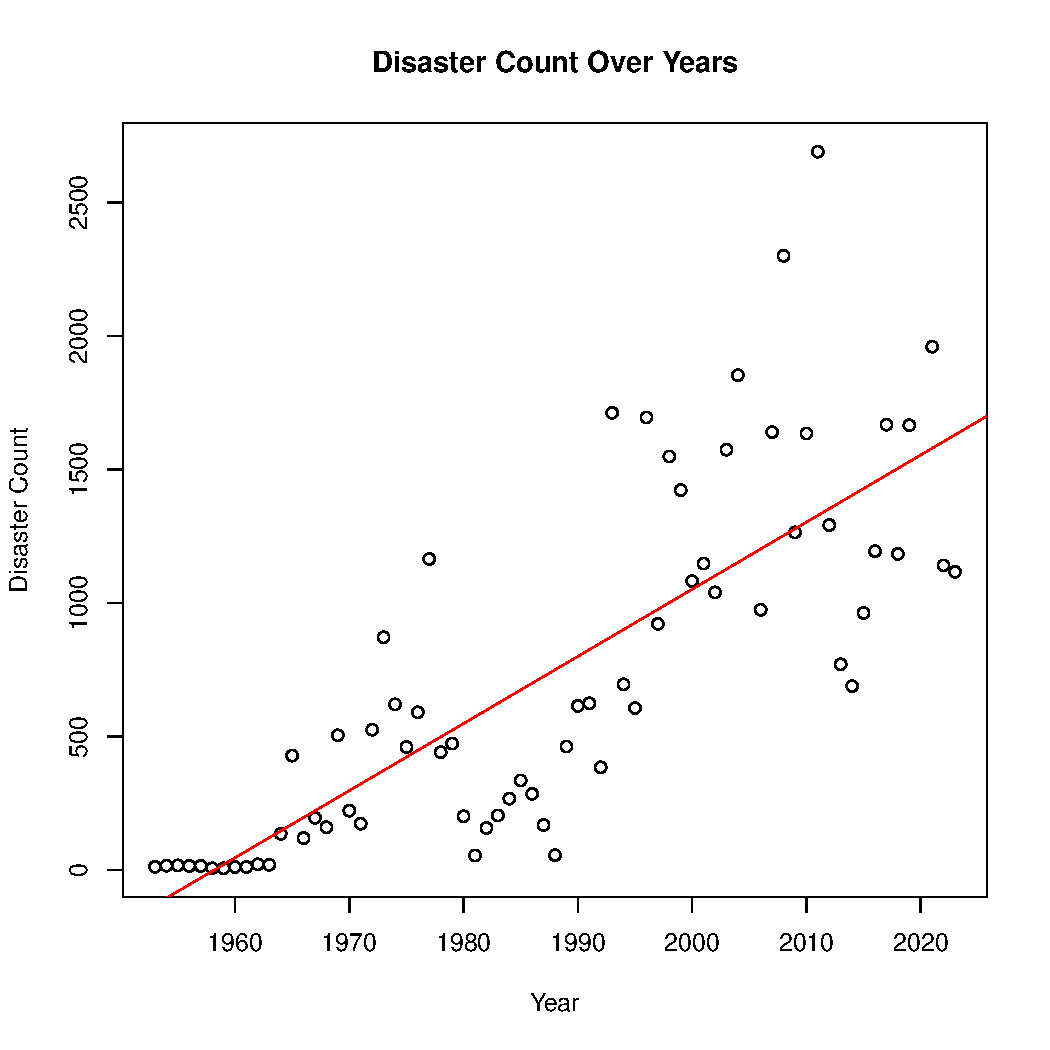
\includegraphics[width=\maxwidth]{figure/q3-1} 
\end{knitrout}

\section*{Prediction Outputs}
Two different methods were used to predict future \textit{DisasterCount} values for the years 2024 to 2035 using a linear model. The results of both methods are closely aligned, with minor variations likely due to rounding procedures:

\begin{enumerate}
    \item \textbf{First Method (Rounded to 1 Decimal Place):} Predicted values range from 1654.9 to 1931.3 disasters for the years 2024 to 2035.
    \item \textbf{Second Method (Rounded to 2 Decimal Places):} Predicted values range from 1654.88 to 1931.32 disasters for the same period.
\end{enumerate}

These predictions indicate an upward trend in \textit{DisasterCount} over the years.

\section*{Model Summary}
The summary of the linear model offers key insights:

\subsection*{Coefficients:}
\begin{itemize}
    \item The intercept is $-49209.962$, implying the model's prediction for \textit{DisasterCount} when \textit{Year} is 0, which is not applicable in this context.
    \item The slope coefficient for \textit{Year} is $25.131$. This indicates an annual increase of approximately 25.131 in \textit{DisasterCount}, as per the model.
\end{itemize}

\subsection*{Statistical Significance:}
Both the intercept and the slope demonstrate statistical significance with a p-value $< 0.001$.

\subsection*{Model Fit:}
\begin{itemize}
    \item The R-squared value is $0.6156$, signifying that approximately 61.56\% of the variability in \textit{DisasterCount} is explained by the year. However, a significant portion of variability remains unexplained.
    \item The Residual Standard Error (RSE) is $409.4$, indicating the average deviation of data points from the fitted line.
\end{itemize}

\subsection*{Residuals:}
The residuals range from $-714.57$ to $1361.83$, suggesting variability around the regression line.

\section*{Interpretation and Considerations}
\begin{itemize}
    \item The model indicates a significant upward trend in disaster counts over the years.
    \item The presence of significant residuals and a R-squared value of $0.6156$ implies that, while there is a discernible trend, other unaccounted factors might also be influencing \textit{DisasterCount}.
    \item Predictions for future years should be approached with caution due to the simplicity of the model and its exclusion of other potential predictive factors.
    \item When interpreting these results and making future decisions, the limitations of a simple linear regression model and the impact of external factors not included in the model should be considered.
\end{itemize}
\end{document}
